\documentclass[14pt]{extbook}
\usepackage{multicol, enumerate, enumitem, hyperref, color, soul, setspace, parskip, fancyhdr} %General Packages
\usepackage{amssymb, amsthm, amsmath, bbm, latexsym, units, mathtools} %Math Packages
\everymath{\displaystyle} %All math in Display Style
% Packages with additional options
\usepackage[headsep=0.5cm,headheight=12pt, left=1 in,right= 1 in,top= 1 in,bottom= 1 in]{geometry}
\usepackage[usenames,dvipsnames]{xcolor}
\usepackage{dashrule}  % Package to use the command below to create lines between items
\newcommand{\litem}[1]{\item#1\hspace*{-1cm}\rule{\textwidth}{0.4pt}}
\pagestyle{fancy}
\lhead{Progress Quiz 4}
\chead{}
\rhead{Version C}
\lfoot{8448-1521}
\cfoot{}
\rfoot{Fall 2020}
\begin{document}

\begin{enumerate}
\litem{
Write the equation of the graph presented below in the form $f(x)=ax^2+bx+c$, assuming  $a=1$ or $a=-1$. Then, choose the intervals that $a, b,$ and $c$ belong to.
\begin{center}
    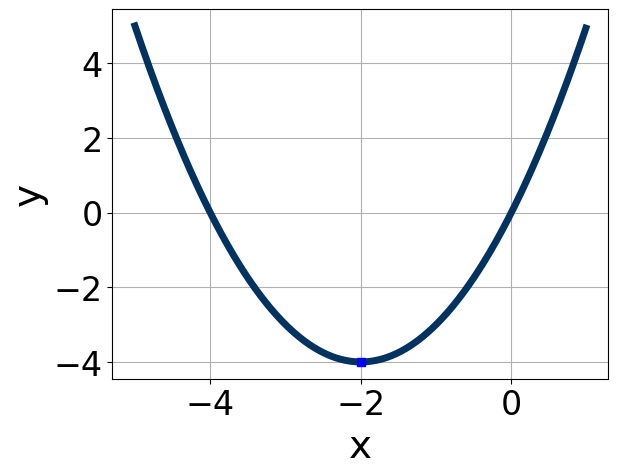
\includegraphics[width=0.5\textwidth]{../Figures/quadraticGraphToEquationCopyC.png}
\end{center}
\begin{enumerate}[label=\Alph*.]
\item \( a \in [-0.3, 1.7], \hspace*{5mm} b \in [-4, -2], \text{ and } \hspace*{5mm} c \in [5, 9] \)
\item \( a \in [-0.3, 1.7], \hspace*{5mm} b \in [4, 6], \text{ and } \hspace*{5mm} c \in [0, 2] \)
\item \( a \in [-2.7, 0.3], \hspace*{5mm} b \in [-4, -2], \text{ and } \hspace*{5mm} c \in [-8, -5] \)
\item \( a \in [-0.3, 1.7], \hspace*{5mm} b \in [-4, -2], \text{ and } \hspace*{5mm} c \in [0, 2] \)
\item \( a \in [-2.7, 0.3], \hspace*{5mm} b \in [4, 6], \text{ and } \hspace*{5mm} c \in [-8, -5] \)

\end{enumerate} }
\litem{
Solve the quadratic equation below. Then, choose the intervals that the solutions $x_1$ and $x_2$ belong to, with $x_1 \leq x_2$.\[ 8x^{2} -18 x -81 = 0 \]\begin{enumerate}[label=\Alph*.]
\item \( x_1 \in [-7.54, -6.19] \text{ and } x_2 \in [1.32, 1.86] \)
\item \( x_1 \in [-18.23, -17.72] \text{ and } x_2 \in [35.81, 36.08] \)
\item \( x_1 \in [-3.28, -1.22] \text{ and } x_2 \in [4.33, 4.53] \)
\item \( x_1 \in [-9.36, -7] \text{ and } x_2 \in [0.79, 1.14] \)
\item \( x_1 \in [-1.69, -0.71] \text{ and } x_2 \in [13.35, 13.95] \)

\end{enumerate} }
\litem{
Graph the equation below.\[ f(x) = -(x-3)^2 - 14 \]\begin{enumerate}[label=\Alph*.]
\begin{multicols}{2}\item 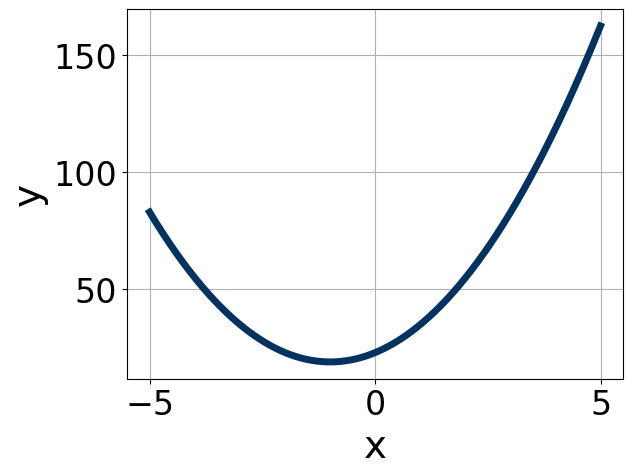
\includegraphics[width = 0.3\textwidth]{../Figures/quadraticEquationToGraphCopyAC.png}\item 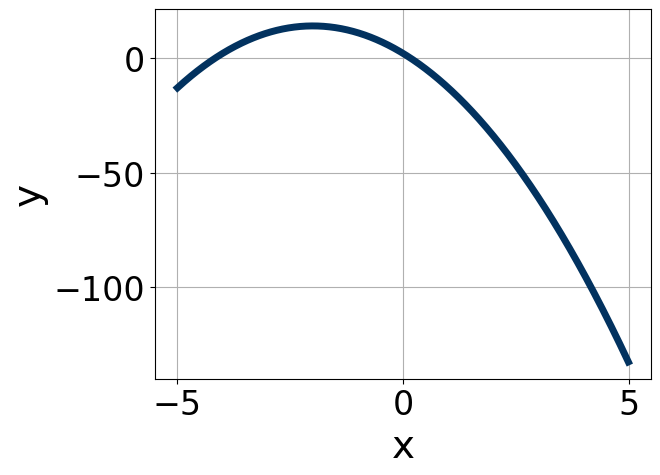
\includegraphics[width = 0.3\textwidth]{../Figures/quadraticEquationToGraphCopyBC.png}\item 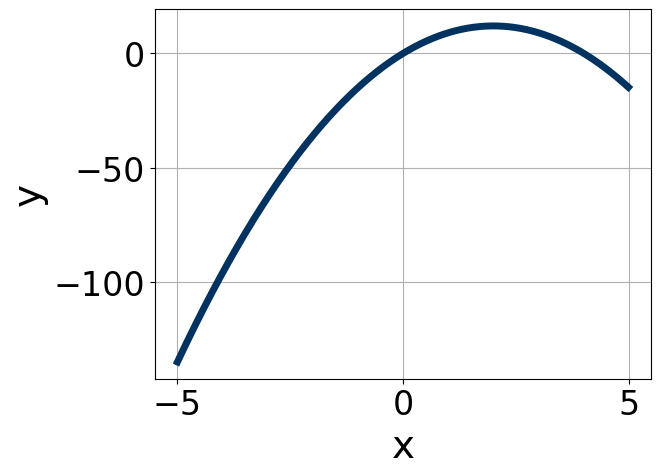
\includegraphics[width = 0.3\textwidth]{../Figures/quadraticEquationToGraphCopyCC.png}\item 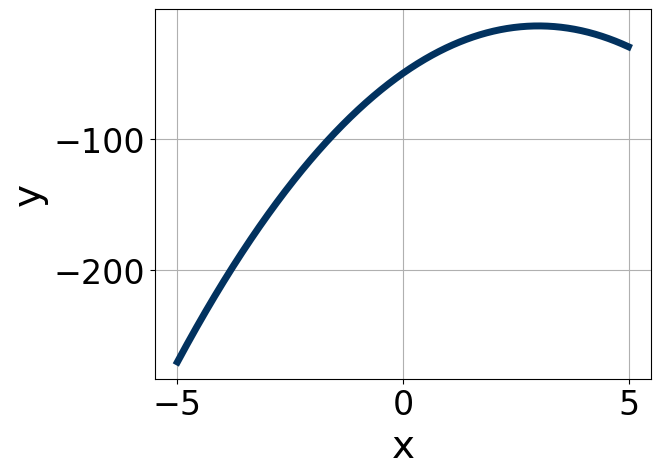
\includegraphics[width = 0.3\textwidth]{../Figures/quadraticEquationToGraphCopyDC.png}\end{multicols}\item None of the above.
\end{enumerate} }
\litem{
Factor the quadratic below. Then, choose the intervals that contain the constants in the form $(ax+b)(cx+d); b \leq d.$\[ 54x^{2} +21 x -20 \]\begin{enumerate}[label=\Alph*.]
\item \( a \in [1.7, 5.9], \hspace*{5mm} b \in [-6, -1], \hspace*{5mm} c \in [11.1, 12.66], \text{ and } \hspace*{5mm} d \in [-1, 10] \)
\item \( a \in [26.2, 29.2], \hspace*{5mm} b \in [-6, -1], \hspace*{5mm} c \in [1.89, 2.44], \text{ and } \hspace*{5mm} d \in [-1, 10] \)
\item \( a \in [6.7, 9.9], \hspace*{5mm} b \in [-6, -1], \hspace*{5mm} c \in [5.04, 6.08], \text{ and } \hspace*{5mm} d \in [-1, 10] \)
\item \( a \in [-1.4, 1.2], \hspace*{5mm} b \in [-27, -23], \hspace*{5mm} c \in [0.8, 1.95], \text{ and } \hspace*{5mm} d \in [43, 47] \)
\item \( \text{None of the above.} \)

\end{enumerate} }
\litem{
Graph the equation below.\[ f(x) = -(x+1)^2 - 14 \]\begin{enumerate}[label=\Alph*.]
\begin{multicols}{2}\item 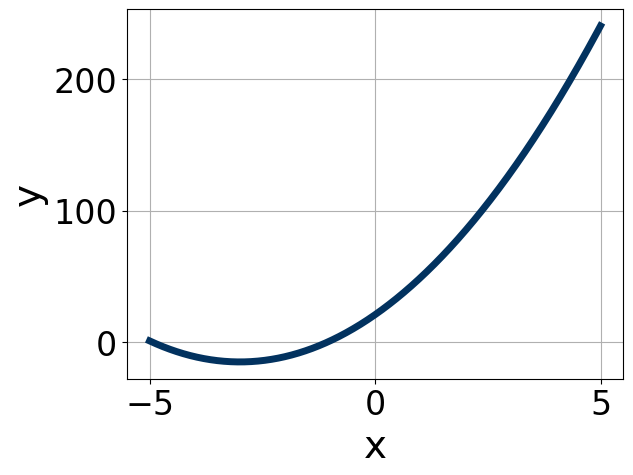
\includegraphics[width = 0.3\textwidth]{../Figures/quadraticEquationToGraphAC.png}\item 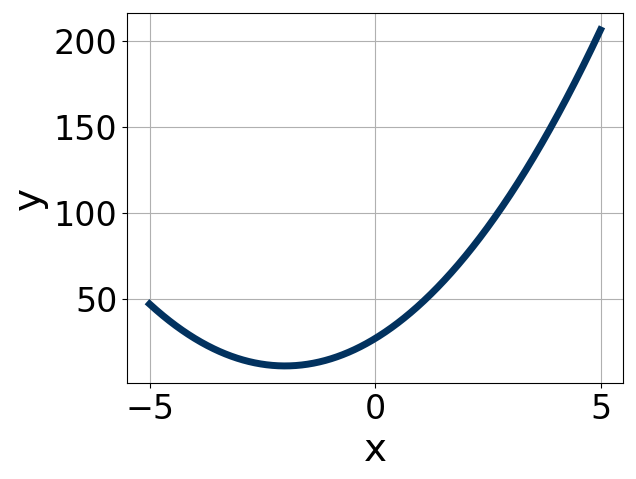
\includegraphics[width = 0.3\textwidth]{../Figures/quadraticEquationToGraphBC.png}\item 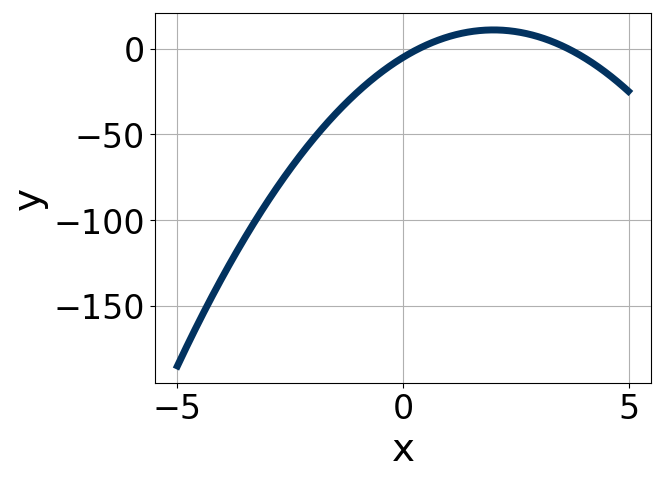
\includegraphics[width = 0.3\textwidth]{../Figures/quadraticEquationToGraphCC.png}\item 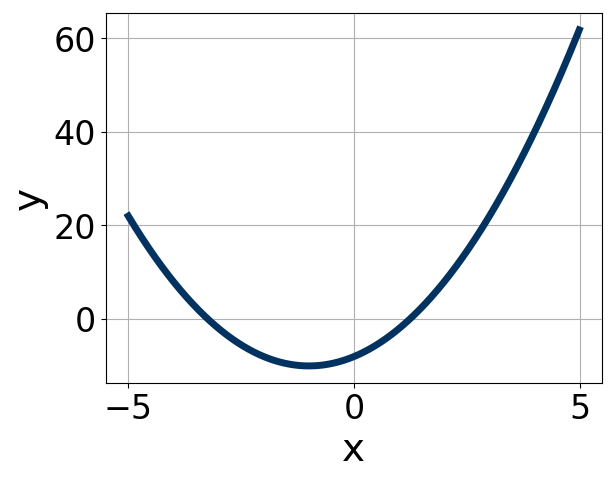
\includegraphics[width = 0.3\textwidth]{../Figures/quadraticEquationToGraphDC.png}\end{multicols}\item None of the above.
\end{enumerate} }
\litem{
Solve the quadratic equation below. Then, choose the intervals that the solutions $x_1$ and $x_2$ belong to, with $x_1 \leq x_2$.\[ 15x^{2} +2 x -24 = 0 \]\begin{enumerate}[label=\Alph*.]
\item \( x_1 \in [-20.14, -19.64] \text{ and } x_2 \in [17.65, 18.51] \)
\item \( x_1 \in [-4, -3.25] \text{ and } x_2 \in [0.3, 0.57] \)
\item \( x_1 \in [-0.9, -0.59] \text{ and } x_2 \in [2.13, 2.4] \)
\item \( x_1 \in [-3.19, -2.43] \text{ and } x_2 \in [0.51, 0.7] \)
\item \( x_1 \in [-1.67, -1.27] \text{ and } x_2 \in [0.88, 1.45] \)

\end{enumerate} }
\litem{
Write the equation of the graph presented below in the form $f(x)=ax^2+bx+c$, assuming  $a=1$ or $a=-1$. Then, choose the intervals that $a, b,$ and $c$ belong to.
\begin{center}
    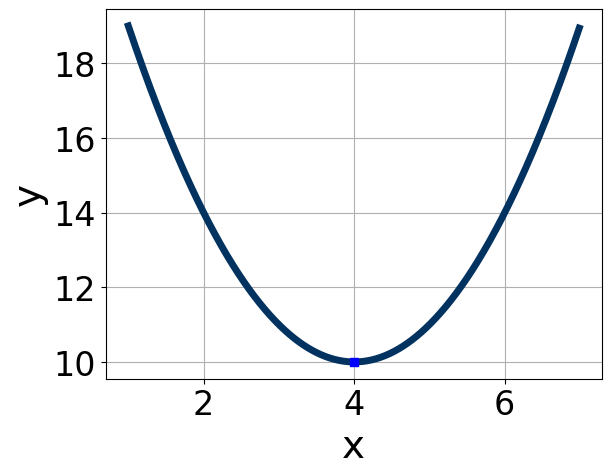
\includegraphics[width=0.5\textwidth]{../Figures/quadraticGraphToEquationC.png}
\end{center}
\begin{enumerate}[label=\Alph*.]
\item \( a \in [-1.5, -0.7], \hspace*{5mm} b \in [-9, -7], \text{ and } \hspace*{5mm} c \in [-18, -16] \)
\item \( a \in [-1.5, -0.7], \hspace*{5mm} b \in [7, 9], \text{ and } \hspace*{5mm} c \in [-18, -16] \)
\item \( a \in [0.5, 1.3], \hspace*{5mm} b \in [-9, -7], \text{ and } \hspace*{5mm} c \in [11, 17] \)
\item \( a \in [-1.5, -0.7], \hspace*{5mm} b \in [-9, -7], \text{ and } \hspace*{5mm} c \in [-15, -11] \)
\item \( a \in [0.5, 1.3], \hspace*{5mm} b \in [7, 9], \text{ and } \hspace*{5mm} c \in [11, 17] \)

\end{enumerate} }
\litem{
Solve the quadratic equation below. Then, choose the intervals that the solutions belong to, with $x_1 \leq x_2$ (if they exist).\[ 10x^{2} +11 x + 2 = 0 \]\begin{enumerate}[label=\Alph*.]
\item \( x_1 \in [-1.9, -0.3] \text{ and } x_2 \in [-0.7, 0.5] \)
\item \( x_1 \in [-0.2, 0.8] \text{ and } x_2 \in [-0.1, 2] \)
\item \( x_1 \in [-7.9, -6] \text{ and } x_2 \in [5.4, 6] \)
\item \( x_1 \in [-10.8, -8.3] \text{ and } x_2 \in [-3, -1.2] \)
\item \( \text{There are no Real solutions.} \)

\end{enumerate} }
\litem{
Solve the quadratic equation below. Then, choose the intervals that the solutions belong to, with $x_1 \leq x_2$ (if they exist).\[ -15x^{2} -13 x + 5 = 0 \]\begin{enumerate}[label=\Alph*.]
\item \( x_1 \in [-22.89, -21.56] \text{ and } x_2 \in [20.33, 21.36] \)
\item \( x_1 \in [-4.56, -4.11] \text{ and } x_2 \in [16.91, 17.37] \)
\item \( x_1 \in [-1.02, 0.09] \text{ and } x_2 \in [1.04, 1.36] \)
\item \( x_1 \in [-2.51, -1] \text{ and } x_2 \in [-0.42, 0.6] \)
\item \( \text{There are no Real solutions.} \)

\end{enumerate} }
\litem{
Factor the quadratic below. Then, choose the intervals that contain the constants in the form $(ax+b)(cx+d); b \leq d.$\[ 16x^{2} +32 x + 15 \]\begin{enumerate}[label=\Alph*.]
\item \( a \in [3.12, 4.94], \hspace*{5mm} b \in [-1, 8], \hspace*{5mm} c \in [3.31, 4.02], \text{ and } \hspace*{5mm} d \in [4, 9] \)
\item \( a \in [-0.6, 1.78], \hspace*{5mm} b \in [7, 18], \hspace*{5mm} c \in [0.86, 1.06], \text{ and } \hspace*{5mm} d \in [17, 25] \)
\item \( a \in [1.38, 2.12], \hspace*{5mm} b \in [-1, 8], \hspace*{5mm} c \in [7.91, 8.45], \text{ and } \hspace*{5mm} d \in [4, 9] \)
\item \( a \in [7.64, 9.22], \hspace*{5mm} b \in [-1, 8], \hspace*{5mm} c \in [1.09, 2.26], \text{ and } \hspace*{5mm} d \in [4, 9] \)
\item \( \text{None of the above.} \)

\end{enumerate} }
\end{enumerate}

\end{document}